\documentclass[12pt,a4paper]{article}
\usepackage[utf8]{inputenc}
\usepackage[german]{babel}
\usepackage[T1]{fontenc}
\usepackage{amsmath}
\usepackage{amsfonts}
\usepackage{amssymb}
\usepackage{graphicx}
\usepackage{siunitx}
\usepackage{float}
\usepackage[left=2cm,right=2cm,top=2cm,bottom=2cm]{geometry}
\author{Gerald}

\begin{document}
\sisetup{separate-uncertainty = true}
	\setlength{\parindent}{0pt} 
	\begin{center}
		{\LARGE Versuchsprotokoll}\\
		\begin{large}
			zum Fortgeschrittenenpraktikum im Bachelorstudiengang Physik\\[0.4cm]
			an der RWTH Aachen\\
			II. Physikalisches Institut A\\[5.5cm]
			\Large\textbf{\textsl{Gasdetektoren und Statistik (T07)}}\\[5.5cm]
			\normalsize\textit{vorgelegt\\von}\\[0.4cm]
			\large{Moritz Berger (355244)\\Gerald Kolter (355005)}\\[2cm]
			\large \textbf{Wintersemester 2017/18}
		\end{large}
	\end{center}
	\newpage
	
	\tableofcontents
	\newpage
	
	
\section{Versuchsziel}
Das Ziel dieses Versuches ist in zwei Teile aufgeteilt.\\
Als erstes sollen die Eigenschaften eines Proportionalzählers und eines Geiger-Müller-Zählrohres untersucht werden. Dazu wird zum einen die Charakteristik, also die Abhängigkeit der Zählrate von der angelegten Spannung, untersucht, um den optimalen Bereich für die Betriebsspannung zu erhalten. Es wird außerdem die Abhängigkeit der Stärke eines Pulses des Proportionalzählers von der Spannung betrachtet und die Tot- und  Erhohlzeit des Geiger-Müller-Zählers bestimmt.\\
Im zweiten Versuchsteil sollen Messungen durchgeführt werden, die verschiedene vorhergesagte Verteilungen bestätigen. Dabei soll eine Gaussverteilung für eine hohe Anzahl an Messungen, eine Poissonverteilung für kleine Messergebnisse und eine Exponetialverteilung für den Abstand zwischen zwei gemessenen Zerfällen untersucht werden. 
\section{Aufbau}
\subsection{Geiger-Müller-Zählrohr}
\subsection{Proportionalzähler}

\section{Durchführung}
\subsection{Geiger-Müller-Zählrohr}
\subsubsection{Charakteristik}
Die Charakteristik wird mithilfe des $_{38}^{90}Sr$-Präparates gemessen. Dabei wird bei eingebrachtem Präparat die Spannung, ausgehend von der Minimaleinstellung von \SI{250}{V}, in \SI{10}{V} erhöht und jeweils über \SI{10}{s} die Anzahl der gemessenen Ereignisse erfasst.\\
Um die Einsatzspannung $U_E$ und die Geiger-Schwelle $U_G$ genauer bestimmen zu können, wurde im entsprechenden Bereich, in dem sich diese Werte befinden, in \SI{2}{V} Schritten statt in \SI{10}{V} Schritten gemessen.
\subsubsection{Totzeit}
Die Totzeit wird über zwei verschiedene Methoden bestimmt.\\
Als erstes wird ein Stever-Diagramm erstellt, an dem man die Tod- und Erhohlungszeit ablesen kann.\\
Als zweites wird sie über eine Totzeitstufe bestimmt.
\subsection{Proportionalzähler}
\subsection{Statistikmessung}
Die Statistikmessungen wurden alle mit dem Geiger-Müller-Zählrohr aufgenommen.
\subsubsection{Poissonverteilung}
Die Zerfälle sind poissonverteilt. Um eine Poissonverteilung auch in den Messdaten beobachten zu können, muss die Messzeit klein gehalten werden (T = 0.3s), da die Verteilung ansonsten in eine Gaußverteilung übergeht. Die Poissonverteilung ist nur für diskrete Werte definiert und hat die Form:
\begin{equation}
P(n) = \dfrac{\mu ^n}{n!} \cdot e^{-\mu}
\end{equation}
\subsubsection{Gaußverteilung}
Da die Zerfälle poissonverteilt sind, muss für die Messung einer Gaußverteilung die Messzeit um Faktor 10 erhöht werden (T = 3s). Die Gaußverteilung hat die Form:
\begin{equation}
P(x) = \dfrac{1}{\sqrt{2 \pi} \sigma} \cdot e^{\frac{(x - \mu)^2}{2 \cdot \sigma ^2}}
\end{equation}
\subsubsection{Exponentialverteilung}
Die Abstände zwischen zwei Zerfällen sind exponentialverteilt. Zur Messung werden mit dem Oszilloskop Bilder gemacht, auf denen mehrere Zerfälle zu sehen sind. Die Exponentialverteilung hat die Form:
\begin{equation}
P(\Delta t) = A \cdot e^{- A \Delta t}
\end{equation}

\section{Ergebnisse}
\subsection{Geiger-Müller-Zählrohr}
\subsubsection{Charakteristik}
\subsubsection{Totzeit}
\subsection{Proportionalzähler}
\subsection{Statistikmessung}

\subsubsection{Poissonverteilung}
\begin{figure}
\centering
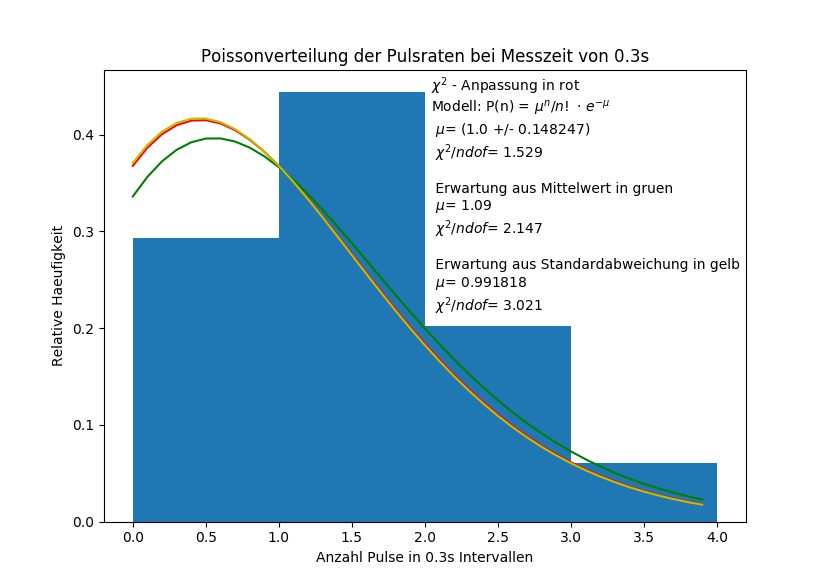
\includegraphics[scale=0.8]{Bilder/poisson.PNG}
\caption{Darstellung der gemessenen Poissonverteilung mit den Erwartungen und der Anpassung.}
\label{fig:Poisson}
\end{figure}


\subsubsection{Gaußverteilung}
\begin{figure}
\centering
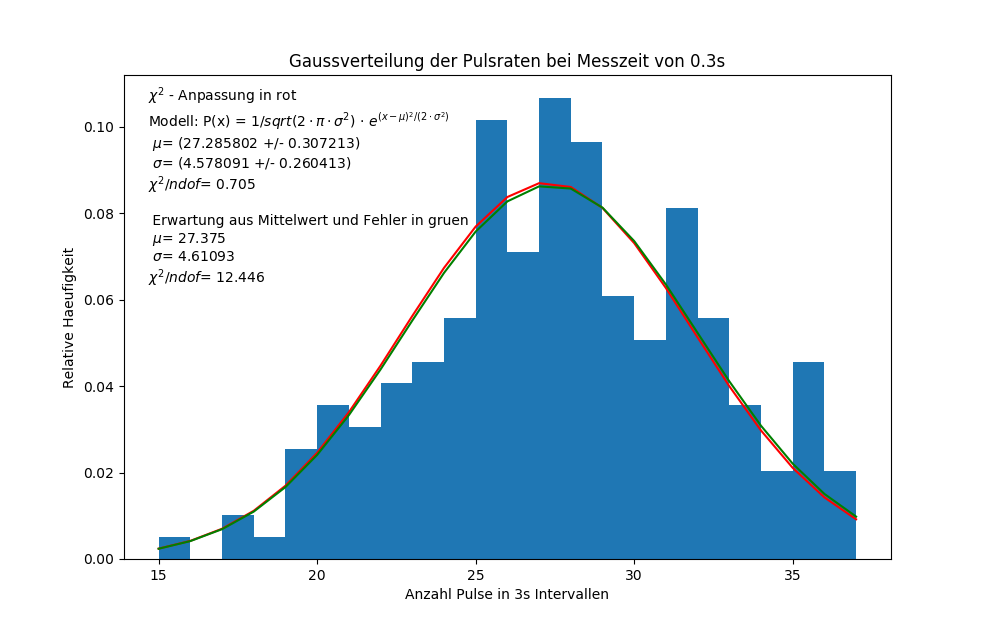
\includegraphics[scale=0.8]{Bilder/gauss.PNG}
\caption{Darstellung der gemessenen Gaußverteilung mit der Erwartung und der Anpassung.}
\label{fig:Poisson}
\end{figure}


\subsubsection{Exponentialverteilung}
\begin{figure}
\centering
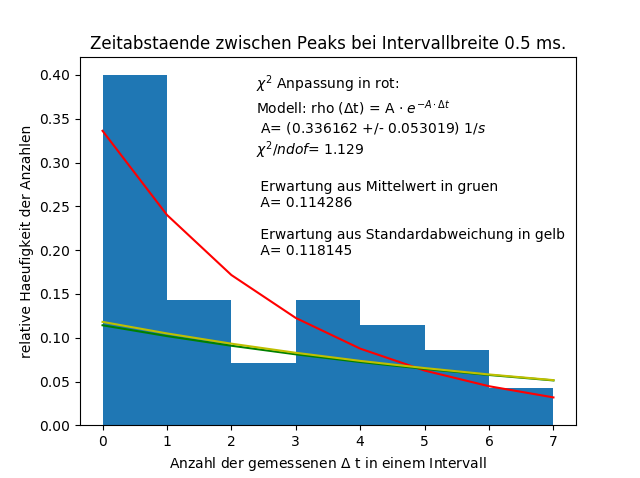
\includegraphics[scale=0.8]{Bilder/Peakabstaende.PNG}
\caption{Darstellung der gemessenen Peakabstände mit den Erwartungen und der Anpassung.}
\label{fig:Poisson}
\end{figure}

\section{Zusammenfassung}




	
\end{document}